\documentclass{article}
\usepackage[margin=1in]{geometry}
\usepackage{amsmath,amsthm,amssymb}
\usepackage{bbm,enumerate,mathtools}
\usepackage{tikz,pgfplots}
\usepackage{chessboard}
\usepackage[hidelinks]{hyperref}
\usepackage{multicol} % Problem 35

\newenvironment{question}{\begin{trivlist}\item[\textbf{Question.}]}{\end{trivlist}}
\newenvironment{note}{\begin{trivlist}\item[\textbf{Note.}]}{\end{trivlist}}
\newenvironment{references}{\begin{trivlist}\item[\textbf{References.}]}{\end{trivlist}}
\newenvironment{related}{\begin{trivlist}\item[\textbf{Related.}]\end{trivlist}\begin{enumerate}}{\end{enumerate}}


\begin{document}
\rating{3}{2}
Consider a spanning tree on the following graph chosen uniformly at random. If
three ``terminal'' vertices are chosen from the tree, there exists a unique ``critical'' vertex
such that every path between any two of the terminal vertices goes through the critical vertex.
\begin{figure}[ht!]
  \centering
  % 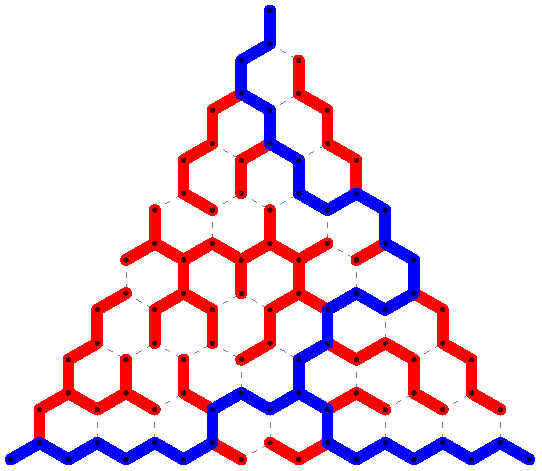
\includegraphics[width=5cm]{assets/126_problem/n_10_1.pdf}
  % 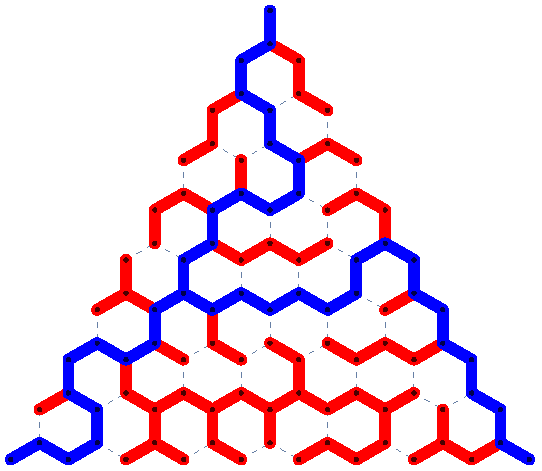
\includegraphics[width=5cm]{assets/126_problem/n_10_2.pdf}
  % 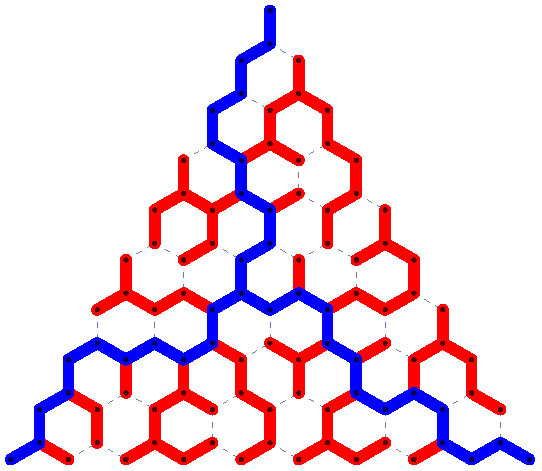
\includegraphics[width=5cm]{assets/126_problem/n_10_6.pdf}
  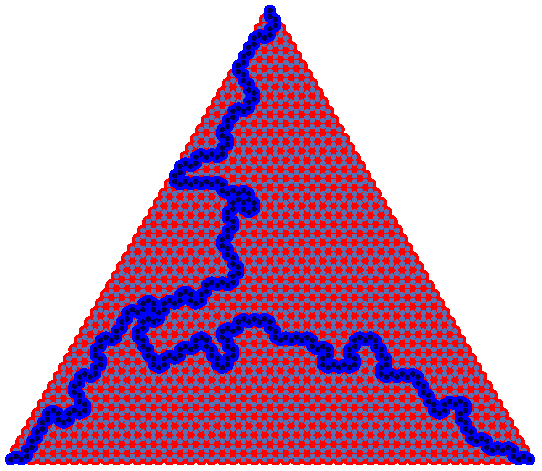
\includegraphics[width=5cm]{assets/126_problem/n_50_1.pdf}
  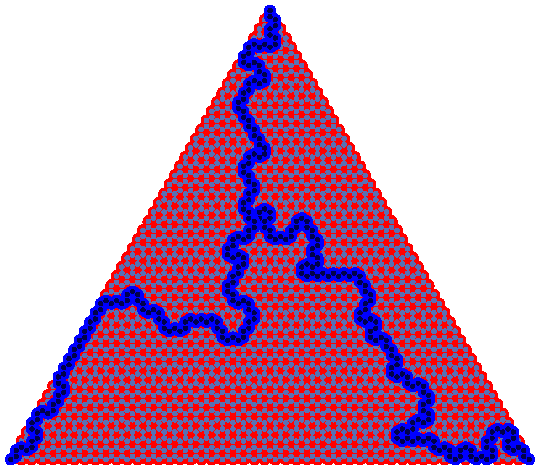
\includegraphics[width=5cm]{assets/126_problem/n_50_4.pdf}
  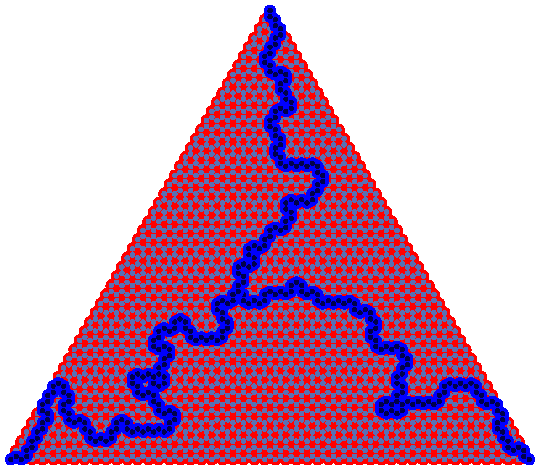
\includegraphics[width=5cm]{assets/126_problem/n_50_6.pdf}
  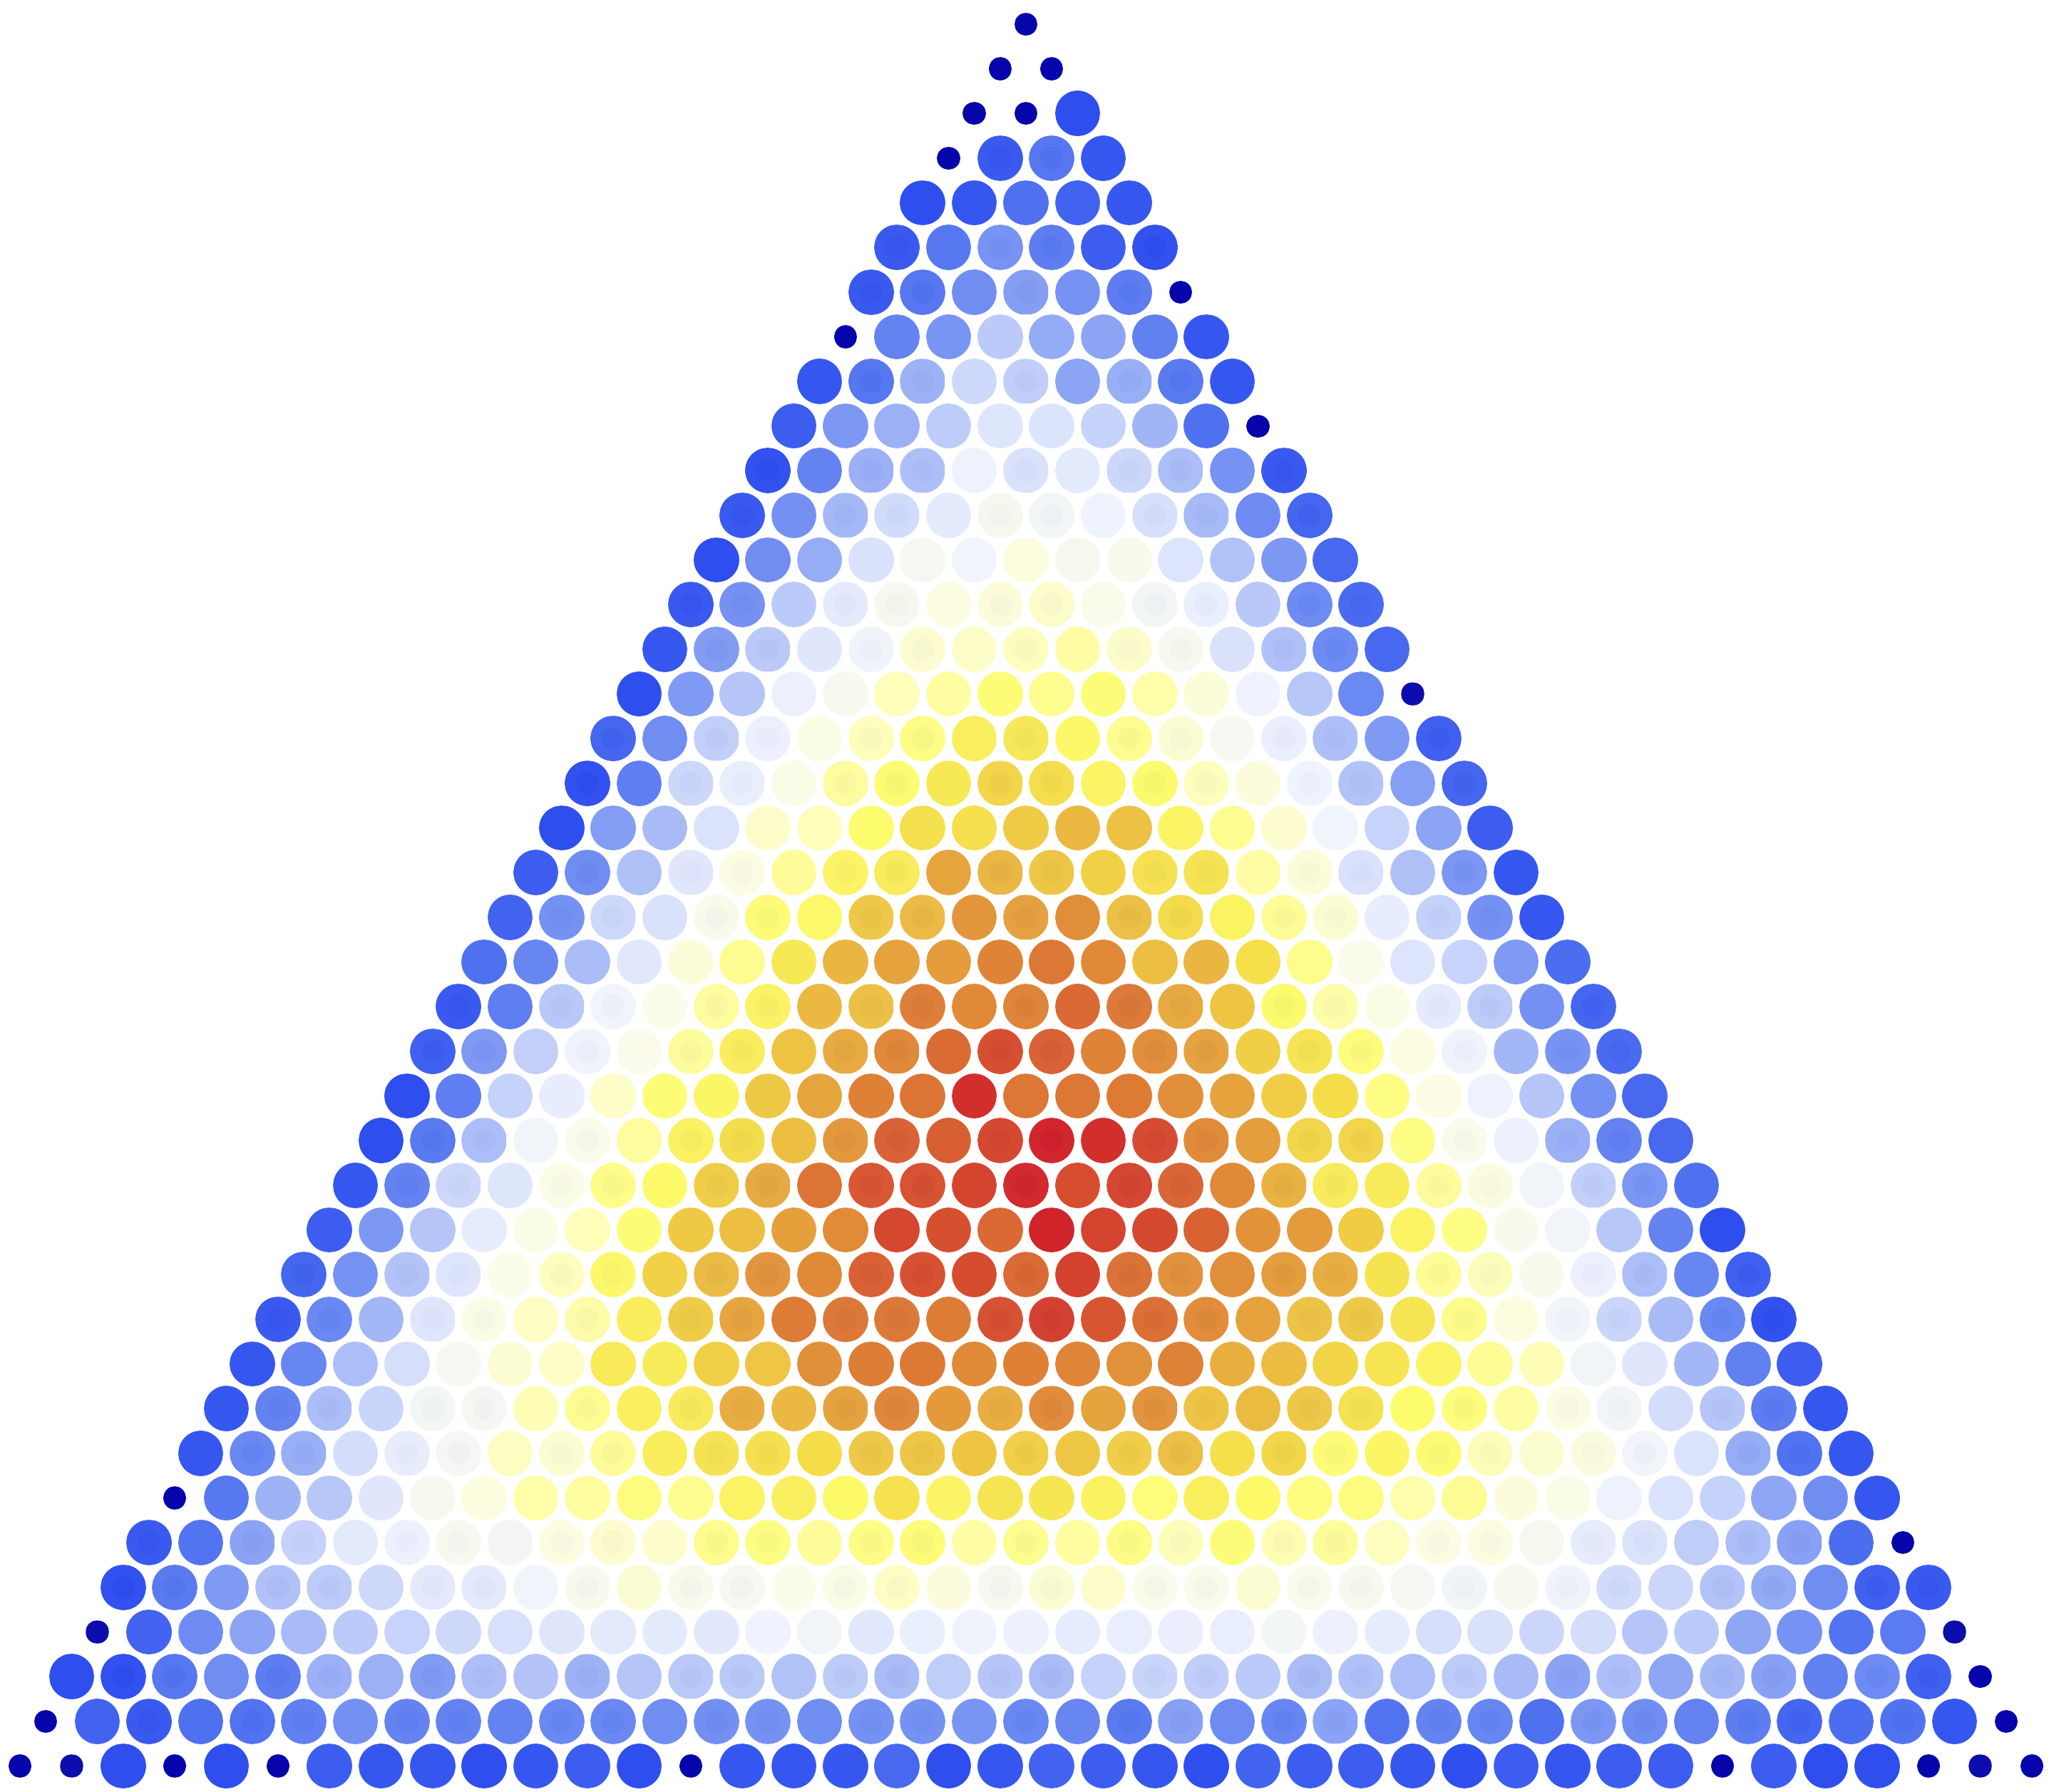
\includegraphics[width=7.5cm]{assets/126_problem/HeatMap.png}
  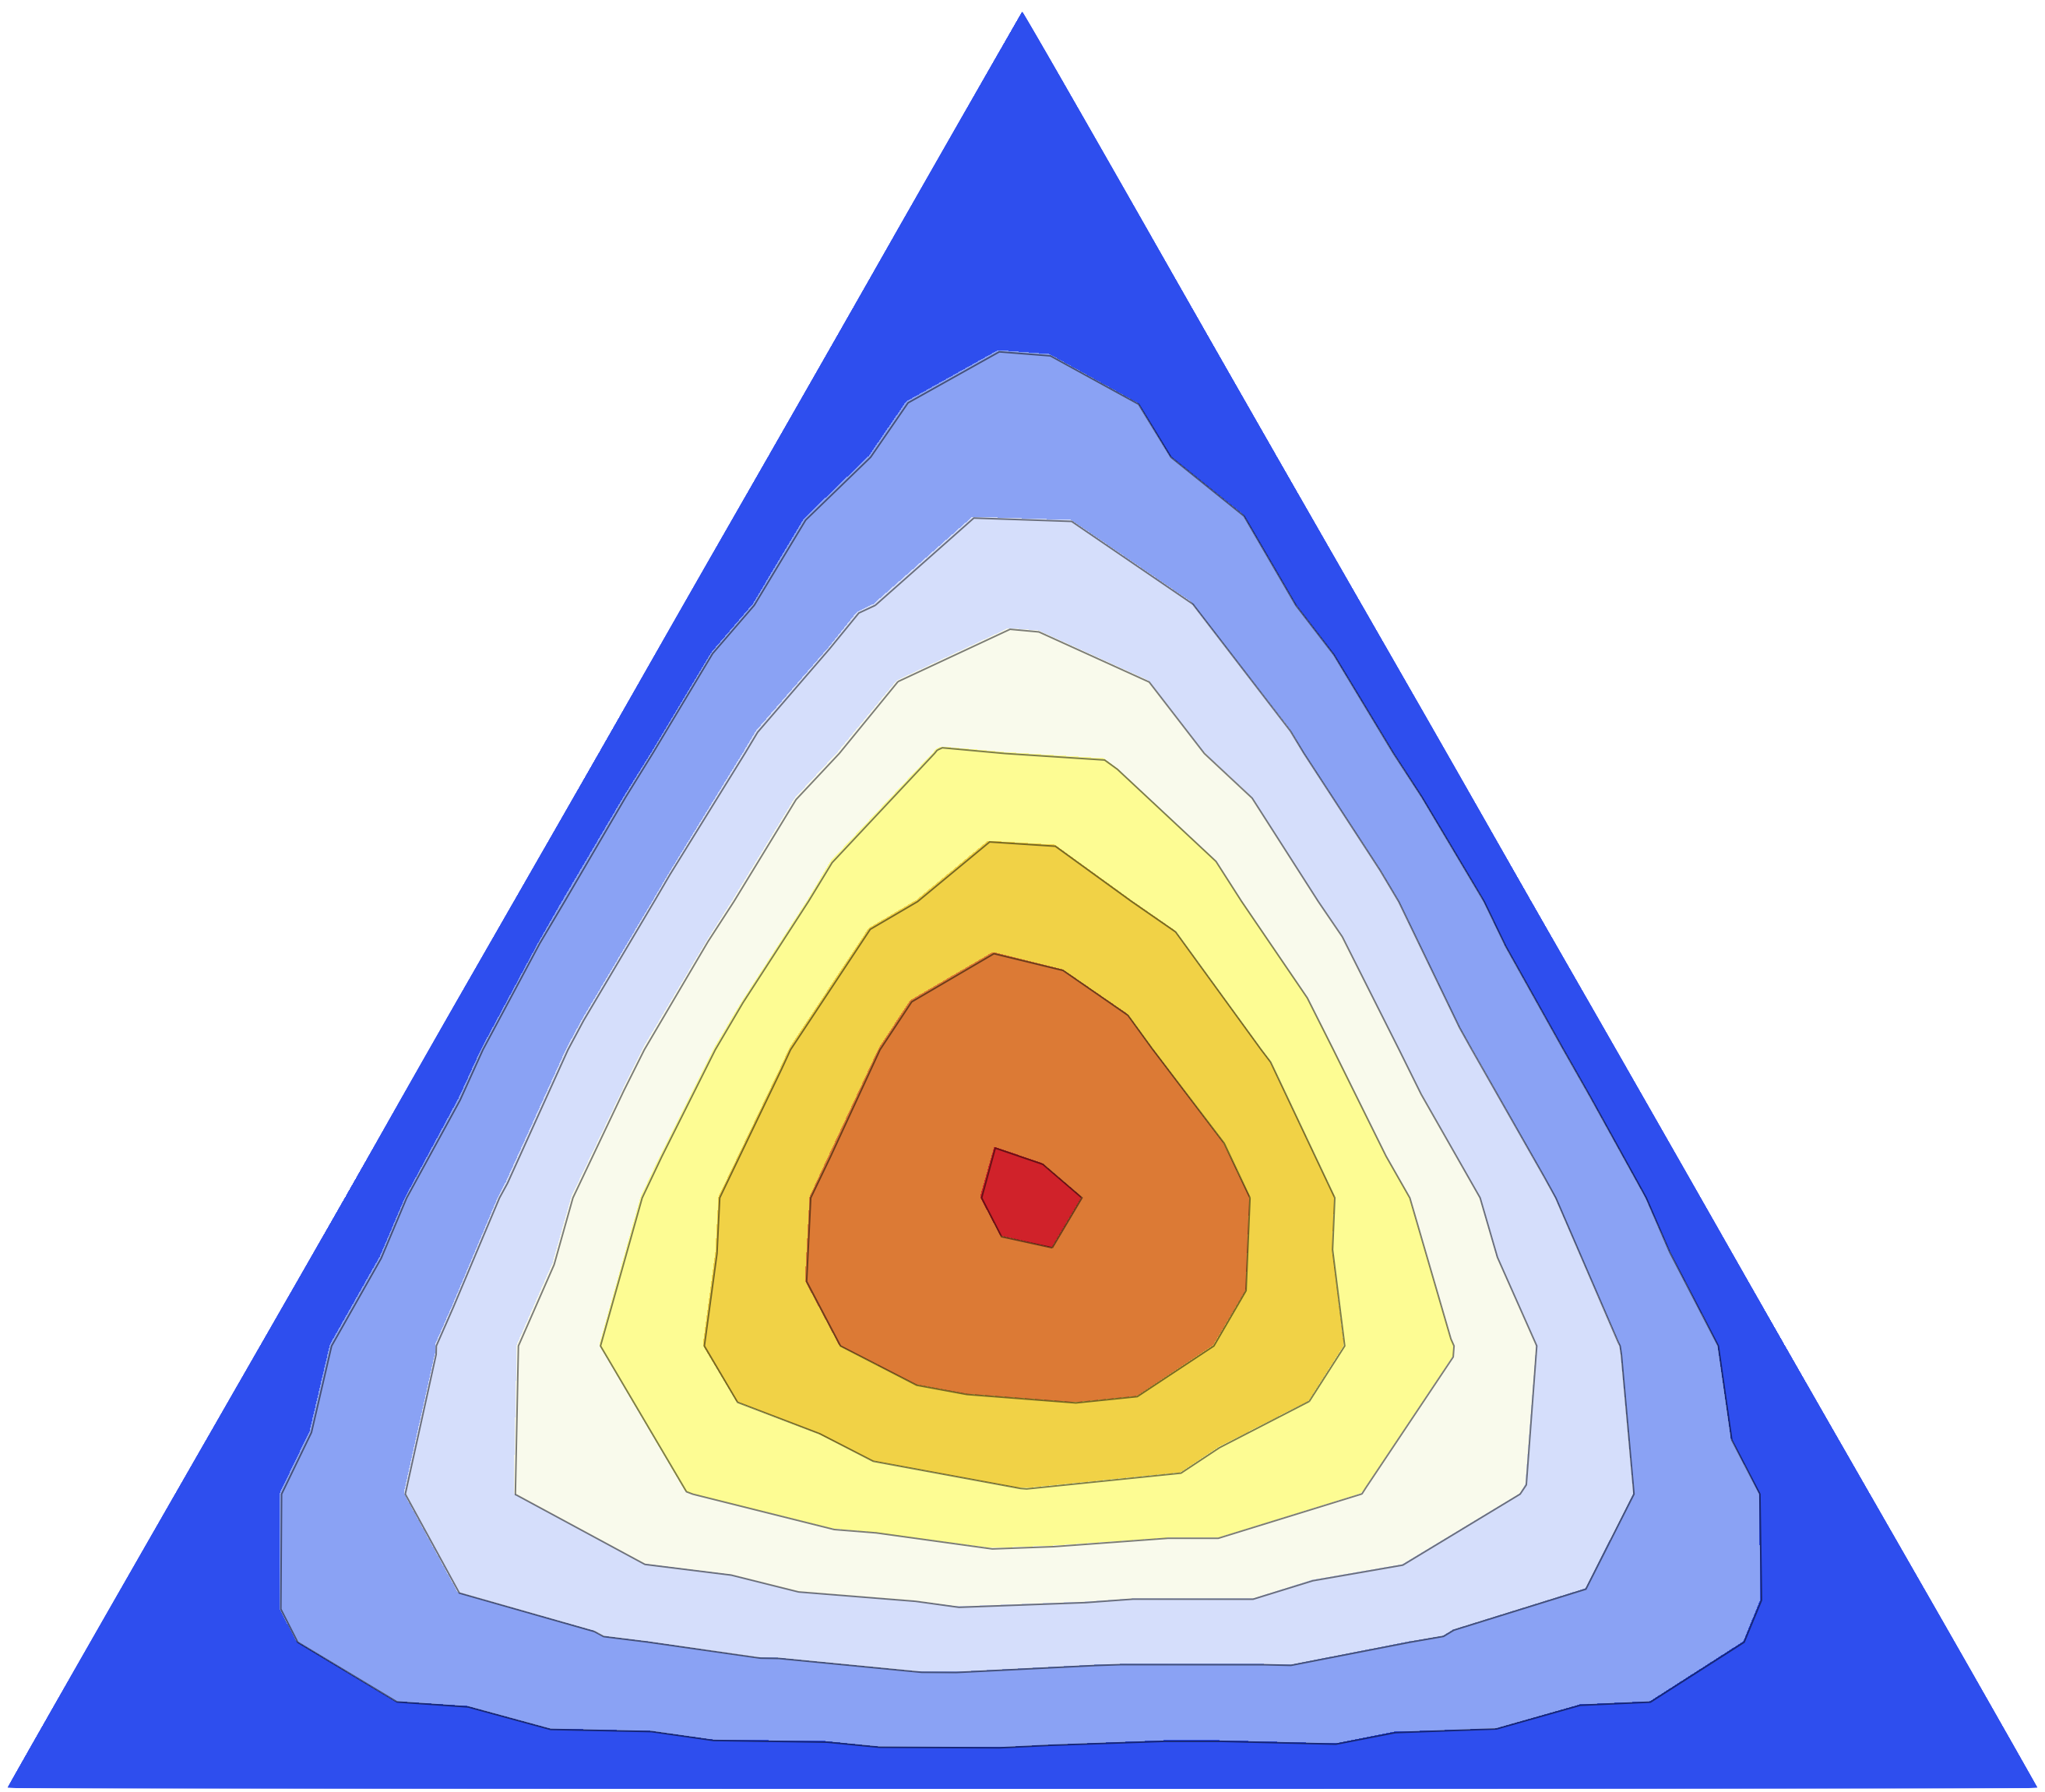
\includegraphics[width=7.5cm]{assets/126_problem/ContourPlot2.png}
  \caption{
    Three examples of critical vertices for $n=50$, and two empirical illustrations of the underlying distribution.
  }
\end{figure}

\begin{question}
  What is the distribution of the terminal vertices as a function of the triangle size?
\end{question}

\begin{related}
  \item If we draw the graphs in the way shown above, scaled so that the bottom
  is unit length, does the limit have a well-defined distribution?
  \item What is the expected value of the total length of the blue path? The distribution?
  \item What is the expected number of regions?
  \item What is the expected ratio of the largest red region to smallest?
\end{related}

\begin{references}
  \item \url{https://oeis.org/A351888}
\end{references}
\end{document}
